Erhält das Elektron einen hinreichend großen Energiebetrag, wird es in einen sog. angeregten Zustand gebracht. Nach einer gewissen Zeit kehrt das Atom in seinen Ruhezustand zurück und die Energie wird als Photon einer bestimmten Wellenlänge emittiert.
Weswegen es bei einem Stoß mit Elektronen dazu kommt, dass die Elektronen - solange sie nicht genug kinetische Energie haben um das Atom anzuregen - nur elastische Stöße mit dem Atom ausführen.\\
Besitzen jedoch die Elektronen genug kinetische Energie um das Atom anzuregen, kommt es zu unealstischen Stößen und das Atom absorbiert einen Teil oder die gesamte Energie des Elektrons.\\

Im Versuch wird ermittelt: Die Energiedifferenz zwischen den Anregungszuständen zweier Atome, die Energie, die nötig ist, um ein Atom zu ionisieren, daher Elektronen aus der Atomhülle herauszuschlagen und die Energieverteilung der austretenden Elektronen.

\begin{figure}[h]
	\centering
	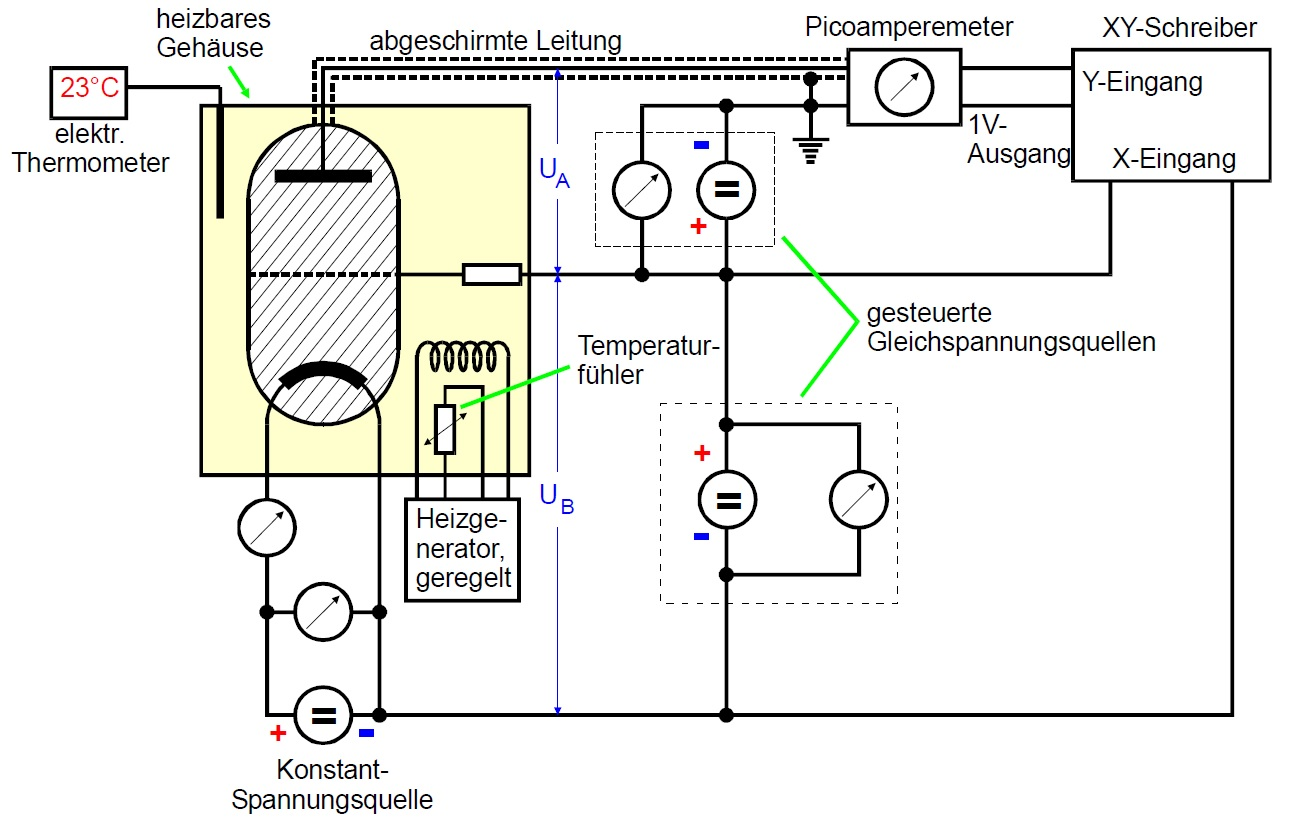
\includegraphics[scale = 0.45]{Grafiken/V601_Abb1.jpg}
	\caption{Versuchsaufbau\cite{V601}}
\end{figure}

Der Franck-Hertz-Versuch besteht grundsätzlich aus einer mit Quecksilberdampf gefüllten Kammer. Man reguliert den Dampfdruck über die innerhalb der Kammer herrschende Temperatur. Diese lässt sich wiederum über einen Heizgenerator steuern.\\
Innerhalb dieser Kammer werden nun von einer Heizkathode ausgehende Elektronen durch eine Beschleunigungsspannung $U_B$ beschleunigt. Die Elektronen erhalten somit die kinetische Energie:
\begin{equation}
E_{kin} = \frac{mv^2}{2} = e_0 U_B
\end{equation}
\\
Am Ende der Kammer befindet sich eine Auffängerelektrode, die die dort auftreffenden Elektronen (als Strom $I_A$) registriert. Vor dieser wird jedoch noch eine Gegenspannung $U_A$ angelegt, so dass nur Elektronen, die

\begin{equation}
E_{kin} \geq e_0 U_A
\end{equation}

erfüllen, die Auffängerelektrode erreichen.\\

Ist die Energie der Elektronen nun kleiner als die Anregungsenergie der Hg-Atome, kommt es lediglich zu elastischen Stößen. Durch die großen Massenunterschiede der beiden Stoßpartner ist die Energieabgabe des Elektrones vernachlässigbar klein. Somit steigt der gemessene Auffängerstrom an, wenn die Beschleunigungsspannung steigt. 
Sobald jedoch die Anregungsenergie erreicht wird, bricht dieser somit auf 0 ein, da die Atome die Energie der Elektronen absorbieren. Auch eine weitere leichte Erhöhung der Energie führt zu keinem Anstieg von $I_A$, da die Energie nicht ausreicht um die Bremsspannung zu überwinden.
\begin{equation*}
E_{kin} - E_1 \leq e_0 U_A
\end{equation*}
Erst bei deutlicher Erhöhung von $U_B$ kommt es zum Ansteigen des Stroms $I_A$.\\
Nach einer weiteren Erhöhung von $U_B$ reicht die Energie der Elektronen für zwei Anregungen, so dass die Kurve wiederum einbricht. Der Abstand U zwischen zwei Maxima gibt die Energie an, die nötig ist um das Atom von einem Zustand in den anderen zu bringen:
\begin{equation}
U_1 := \frac{1}{e_0}(E_1 - E_0)
\end{equation}

\begin{figure}[h]
	\centering
	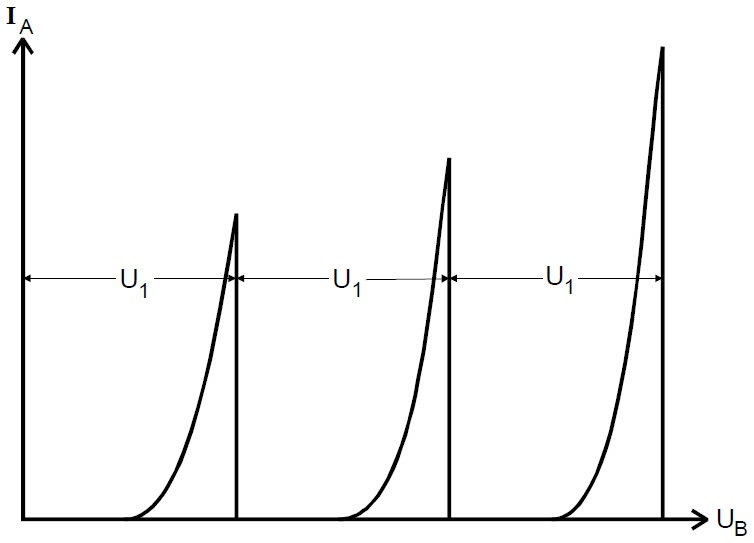
\includegraphics[scale = 0.5]{Grafiken/V601_Abb2.jpg}
	\caption{Idealisierte Franck-Hertz-Kurve\cite{V601}}
\end{figure}
\newpage
\subsection{Einflüsse auf die Gestalt der Kurve}
Es gibt allerdings noch weitere Effekte, die die vorher beschriebene, idealisierte Gestalt der Franck-Hertz-Kurve beeinflussen.

\subsubsection{Einfluss des Kontaktpotentials}
Um hohe Elektronenemissionsraten zu erreichen, verwendet man für Glühdraht und Beschleunigungselektrode Materialien, die beide unterschiedliche Austrittsarbeiten besitzen, wobei der Glühdraht die deutlich kleinere Austrittsarbeit besitzen sollte. Damit kommt es durch die verschieden Potentiale zu einer Verschiebung der Franck-Hertz-Kurve um das Kontaktpotential:

\begin{equation}
K = \frac{\Phi_B - \Phi_G}{e_0}
\end{equation}

\subsubsection{Einfluss des Energie-Spektrums der Elektronen}
In Materialien besitzen nicht alle Elektronen den gleichen Energiewert, sondern eine statistische Energieverteilung, denn die Elektronen treten mit unterschiedlichen Geschwindigkeiten bzw. kinetischen Energien, aus dem Glühdraht aus.\\
Dies führt dazu, dass es keine Unstetigkeiten in der Kurve gibt, sondern die Abfälle auf $I_A$ = 0 mit einer endlichen Steigung geschehen und sich einem Stromminimum nähert.\\

\subsubsection{Einfluss des Dampfdrucks}
Um aussagekräftige Kurven zu erhalten, ist es nötig die Stoßwahrscheinlichkeit der Elektronen mit den Hg-Atomen ausreichend hoch zu halten. Dazu ist es nötig, dass die mittlere freie Weglänge $\overline{w}$ klein gegen den Abstand $a$ der Glühkathode zur Auffängerelektrode ist.\\
Dabei hängen $\overline{w}$ und der Sättigungsdruck über
\begin{equation}
\label{eq:Theorie_Weglaenge}
\overline{w} [cm] = \frac{0,0029}{p_{sät}} \quad [p \, \text{in} \, mbar]
\end{equation}
zusammen.\\

Wobei gilt
\begin{equation}
\label{eq:Theorie_Dampfdruck}
p_{sät}(T) = 5,5 \cdot 10^{7} \exp(-6876/T)\quad [p \, \text{in} \, \si{\milli\bar}, \, T \, \text{in} \, \si{\kelvin}]
\end{equation}
$\overline{w}$ sollte dabei um einen Faktor 1000 bis 4000 kleiner sein als der Abstand $a$.
